%数理科学研究会
%TeXサンプル
\documentclass[a4paper, 12pt, dvipdfmx]{jsarticle}
\usepackage{otf} %otfパッケージを読み込むことで様々な問題を回避できる
\usepackage[T1]{fontenc} %T1エンコードにすることで様々な問題を回避できる
\usepackage{lmodern} %フォントサイズの問題を回避
\usepackage{exscale} %大型演算子の問題を回避
\usepackage{etex}
\usepackage[dvipdfm, truedimen, top=25truemm, hmargin=25truemm, bottom=25truemm]{geometry} %用紙サイズの設定

%定理環境の設定
\usepackage{amsthm}
\theoremstyle{definition}
\newtheorem{theorem}{定理}[section]
\newtheorem{definition}[theorem]{定義}
\newtheorem{lemma}[theorem]{補題}
\newtheorem{axiom}[theorem]{公理}
\newtheorem{proposition}[theorem]{命題}
\newtheorem{corollary}[theorem]{系}
\newtheorem{example}[theorem]{例}
\newtheorem*{theorem*}{定理}
\newtheorem*{definition*}{定義}
\newtheorem*{lemma*}{補題}
\newtheorem*{axiom*}{公理}
\newtheorem*{proposition*}{命題}
\newtheorem*{corollary*}{系}
\newtheorem*{example*}{例}
\renewcommand\proofname{\bf 証明}

%スタイルファイルを追加したい場合は以下のように書く
\usepackage{graphicx}
\usepackage{amsmath,amssymb}
\usepackage{eclbkbox}
\usepackage{tikz}

%\newcommandでマクロを定義できる
\newcommand{\macrotest}{\LaTeX のマクロは便利}
\newcommand{\PD}[2]{\frac{\partial {#1}}{\partial {#2}}}%引数もとれる

%日付を和暦にするには下のようにすれば良い.
\和暦

\title{数理科学研究会\TeX サンプル}
\date{\today}
\author{XY99999 \quad 芝浦 太郎}
\begin{document}
\maketitle


%%%%%%%%%%%%%%%%%%%%%%%%%%%%%%%%%%%%%%%%%%%%%%%%%%%%%%%%%%%%%%%%%%%%%
%%%%%%%%%%%%%%%%%%%%%%%%%%%%%%%%%%%%%%%%%%%%%%%%%%%%%%%%%%%%%%%%%%%%%
%以下サンプル%ここから書き始めてください

\section{節}
\subsection{小節}
\subsubsection{小々節}

\subsection{オイラー}
$e^{i\pi}+1=0$という等式は, オイラーの等式と呼ばれています.
オイラーは式 (\ref{eq:Basel})を示しました.
%\labelと\refを使うと自動で番号を振ってくれる
\begin{align}
    \frac{\pi^2}{6}=\sum_{n=1}^\infty \frac{1}{n^2} \label{eq:Basel}
\end{align}
オイラーはさらに
\begin{align*}
    \frac{\pi^4}{90}&=\sum_{n=1}^\infty \frac{1}{n^4},\\
    \frac{\pi^6}{945}&=\sum_{n=1}^\infty \frac{1}{n^6}
\end{align*}
という式も示しました.

\subsection{フェルマー}
\begin{theorem}[フェルマーの小定理]
    任意の素数$p$と, 任意の$a\in \mathbb{Z}$に対して, $a^p\equiv a \pmod{p}$が成り立つ.
\end{theorem}
\begin{proof}
    うんたらかんたら.
    よって, 示せた.
\end{proof}
\begin{theorem}[フェルマーの最終定理]
    任意の整数$n\geq 3$に対して, $x^n+y^n=z^n$となる自然数の組$(x,y,z)$は存在しない.
\end{theorem}
\begin{proof}
    うんたらかんたら.
    余白が狭すぎる.
\end{proof}

\section{色々}
数学の文章では, ``、''や``。''でなく``,''と``.'' (共に半角)を使う.
また, ``,''と``.''の後には半角スペースを入れる.

表を入れてみました (表\ref{tab:test}).
図も入れてみました (図\ref{fig:test}).

\begin{table}[h]
    \centering
    %表のキャプションは表の上に, 図のキャプションは図の下に付ける
    \caption{表のテスト}
    \label{tab:test}
    \begin{tabular}{|c||cc|}
        \hline
        a & b & c\\ \hline \hline
        d & e & f\\
        g & h & i\\ \hline 
    \end{tabular}
\end{table}

\begin{figure}[h]
    \centering
    %使い方はhttp://perikanfan.web.fc2.com/Manual.pdf 等参照.
    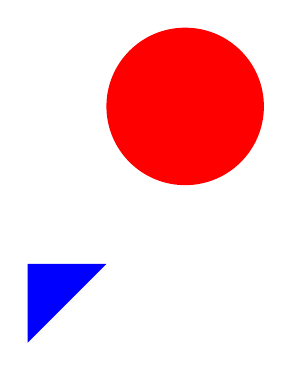
\begin{tikzpicture}
        \fill[blue] (0,0) -- (0,1) -- (1,1) -- (0,0);
        \fill[red] (2,3) circle [radius=1];
    \end{tikzpicture}
    \caption{図のテスト}
    \label{fig:test}
\end{figure}

$\langle a, b\rangle$は\verb|$\langle a, b\rangle$|と書く.
(\verb|$<a, b>$|では$<a, b>$となってしまう.)

本当に\macrotest.
\begin{align*}
    \PD{u}{t}+c\PD{u}{x}=0.
\end{align*}

\begin{thebibliography}{1}
    %著者, タイトル, 出版社, 現在の版の第1刷が発行された年.
    \bibitem{TeX} Donald E.Knuth 著, 鷺谷好輝 訳, \TeX ブック コンピュータによる組版システム, アスキー, 1989.
    \bibitem{LaTeX} 奥村晴彦, 黒木祐介, [改訂第7版] \LaTeXe 美文書作成入門, 技術評論社, 2017.
\end{thebibliography}
\end{document}
